
%(BEGIN_QUESTION)
% Copyright 2012, Tony R. Kuphaldt, released under the Creative Commons Attribution License (v 1.0)
% This means you may do almost anything with this work of mine, so long as you give me proper credit

Write integral expressions for each of the shaded areas on this graph, assuming both areas have {\it negative} values:

$$\includegraphics[width=15.5cm]{i01908x01.eps}$$

\underbar{file i01908}
%(END_QUESTION)





%(BEGIN_ANSWER)

Blue-shaded area:

$$\int_{-9}^{-5} y \> dx \hskip 30pt \hbox{ . . . or . . .} \hskip 30pt \int_{-5}^{-9} -y \> dx$$

\vskip 30pt

Red-shaded area:

$$\int_{1}^{8.5} -y \> dx \hskip 30pt \hbox{ . . . or . . .} \hskip 30pt \int_{8.5}^{1} y \> dx$$

%(END_ANSWER)





%(BEGIN_NOTES)


%INDEX% Mathematics, calculus: integral (defined in a graphical sense)

%(END_NOTES)


